\subsection{Decision 8: Interaction with ticket scanners}

\subsection*{Status}
Accepted.

\subsection*{Architectural Summary}
\begin{tabular}{|p{3.5cm}|p{10.5cm}|}
    \hline
    \textbf{In the context of} & turnstile interaction with the TRiP system, \\
    \hline
    \textbf{Facing} & the passengers' request for a seamless travel experience and tycoon need to admit only authorized passengers in their stations, \\
    \hline
    \textbf{To achieve} & high availability, security in sensitive data communication, many options adapted to different passengers needs, \\
    \hline
    \textbf{We considered} & Option 1: Add a ticket checker and a user state modules to authorize passengers; Option 2: Allow fillable cards, account cards and tickets, not bank cards;\\
    \hline
    \textbf{And decided for} & Option 1: Add a ticket checker and a user state modules to authorize passengers;\\
    \hline
    \textbf{Because} & Not allowing bank cards would make us lag behind with respect to modern train payment systems that allow high usability for tech-savy passengers, \\
    \hline
    \textbf{Accepting} & The need for an offline mode in case the network fails, possible latency. \\
    \hline
\end{tabular}
\subsection*{Concern}
Passengers want a seamless travel experience, without being mistakenly blocked at the turnstiles.
Tycoons want to admit only paying passengers in trains, avoiding controllers costs.
Turnstiles need to communicate with the system to ensure correct and quick verification of the requisites to be allowed in the station.

\subsubsection*{User Stories}
The decision on how turnstiles interact with the payment system is integral to ensuring a seamless travel experience and securing access to train areas. Below, we detail specific user stories connected to this architectural decision, highlighting the requirements and expectations from various stakeholders.

\begin{enumerate}[noitemsep]
    \item \userStoryOne,
    \item \userStoryTwentySix,
    \item \userStoryTwentySeven,
    \item \userStoryTwentyThree,
\end{enumerate}

These user stories collectively highlight the diverse requirements for the turnstile and payment system interaction, from seamless access and real-time information integration to flexibility in handling various ticketing formats and system updates.
The problem can be made more abstract, as the interaction with the turnstile can be similar to the following interactions:
\begin{itemize}
    \item interaction with a controller who scans the ticket or any proof of subscription.
    \item interaction with a scanner onboard a bus.
\end{itemize}

\subsection*{Context}

Most stations, expecially the big ones, have turnstiles to avoid people without tickets to enter the trains area.
The turnstiles should communicate with the system to ensure this. A decision should be taken on who to admit in the station.
This logic could be provided by the station manager or by the tycoons, or even by TrIP managment.
How do the passenger input its ticket or subscription or prepaid card to the turnstile?
How does the turnstile communicate with the system to verify if the passenger has the right to enter the station?

\subsection*{Criteria}
\begin{itemize}
    \item \textit{Usability and functionality}: Allow passengers to scan tickets or multiplatform travel cards (if they exists) at turnstiles.
    \item \textit{Safety}: Don't allow people without the appropriate tickets or subscriptions or cards.
    \item \textit{Availability and performance}: Let passenger quickly open turnstiles when they are authorized.
    \item \textit{Functionality}: Possibly allow people to scan when they enter and when they exit and calculate a fare (this might depend on agreements between tycoons). 
    \item \textit{Functionality}: Possibly communicate station usage data to the system.
    \item \textit{Functionality}: Possibly allow credit/debit card scan.
    \item \textit{Functionality}: Allow balance check for charged cards.
\end{itemize}
    

\subsection*{Option 1: Add a ticket checker and a user state module to authorize passengers}
After scanning a ticket or badge, the user state should be updated, in order to calculate the fare price for fillable card holders or for the scanning of bank cards (debit credit).
The ticket or badge should be checked by the single ticket checker module or by the account management to insure consistency.
In case of the scanning of bank cards, the user state module needs to communicate with payment management, in order to proceed with the actual payment.
The scanning of bank cards and fillable cards create the needs for a calculation of appropriate revenue share between different tycoon. This should be the topic of a future decision or might be incorporated in this one.
\begin{figure}[ht]
    \centering
    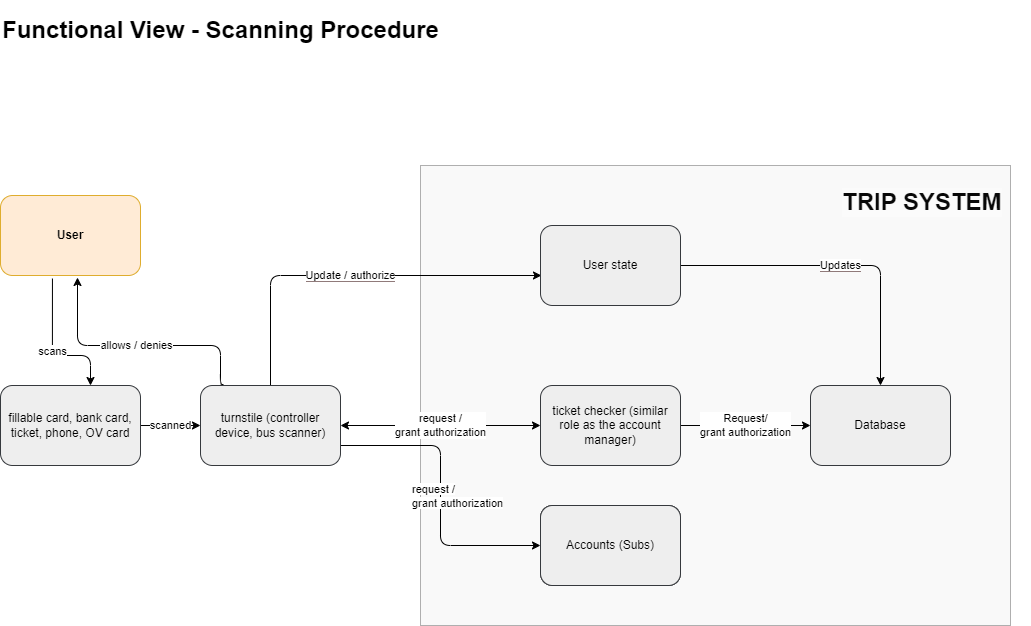
\includegraphics[width=\textwidth]{drawings/views_draft2/functional_view turnstiles.png}
    \caption{Interaction with a ticket scanner.}
    \label{fig:ticket_scanner}
\end{figure}

\subsection*{Option 2: Allow fillable cards, account cards and tickets, not bank cards}
Not allowing bank cards at turnstiles simplifies the job of turnstiles.
Also, how can a controller check if the traveller have scanned a bank card when entering the turnstile?
We can have the turnstile print a ticket with a barcode or QR code.
This way all the relevent information is contained in the card or ticket and no on-line check is needed. 

\subsection*{Decision}
We choose Option 1, as refusing bank cards checking would hinder usability for the passengers. It would make us lag behind with respect to other train payments systems. 
The security risk that this poses can be mitigated by applying an encryption tactic (this will be explained in more detail in the information viewpoint).
An offline mode needs to be detailed to face Event 2 (possible network disruptions in stations), this will be explianed in the concurrency viewpoint.

\subsection*{Positive Consequences}
\begin{itemize}
    \item Enhances security by ensuring only authorized passengers can access services.
    \item Improves passenger experience with seamless turnstile interaction.
    \item Supports real-time updates for station managers, enhancing operational efficiency.
    \item Integrates with modern payment systems, offering convenience to tech-savvy passengers.
    \item Provides for an offline mode, ensuring system reliability in case of network failures.
\end{itemize}

\subsection*{Negative Consequences}
\begin{itemize}
    \item Introduces system complexity and potential integration challenges.
    \item Creates dependency on external payment systems, raising operational risks.
    \item Incurs significant operational costs for implementation and maintenance.
    \item Raises data privacy and security concerns due to sensitive information handling.
    \item Complicates the revenue-sharing model among tycoons, requiring detailed negotiations.
\end{itemize}